\section{Introduction}

Nowadays many malwares use HTTP protocol to connect to suspicious host or send the sensitive data because it's a commonly open channel in the networks. Therefore malwares try to hide in the normal traffic to evade the detections.

As in Analyzing HTTP User Agent Anomalies for Malware Detection \cite{kheir2013analyzing}, they claim with up to 60\% of malware showing at least one outgoing HTTP connection. There are differen research indicate there are many botnet using HTTP protocl to communicate with the C\&C server for waiting command instead of IRC channel \cite{gu2008botsniffer}.

Our system use fingerprint to detect outbound http traffic. The idea come from DECANTeR.

But the main concept is around the HTTP headers. But as we know, we can use some tool or library to eaily modify the HTTP headers. Some research indicate some malwares also use modified HTTP header to evade the latest detections system. In the [Malware Detection Using HTTP User-Agent Discrepancy Identification] point out there are 40\% malwares using browser-like user-agent since browser's connection behaviors are more complex than application connections.

Thence we represent a detection system to captical these Counterfeit abnormal traffic. We evaluate our system's validity through simulated dataset and real world dataset.

\begin{figure}[!t]
\centering
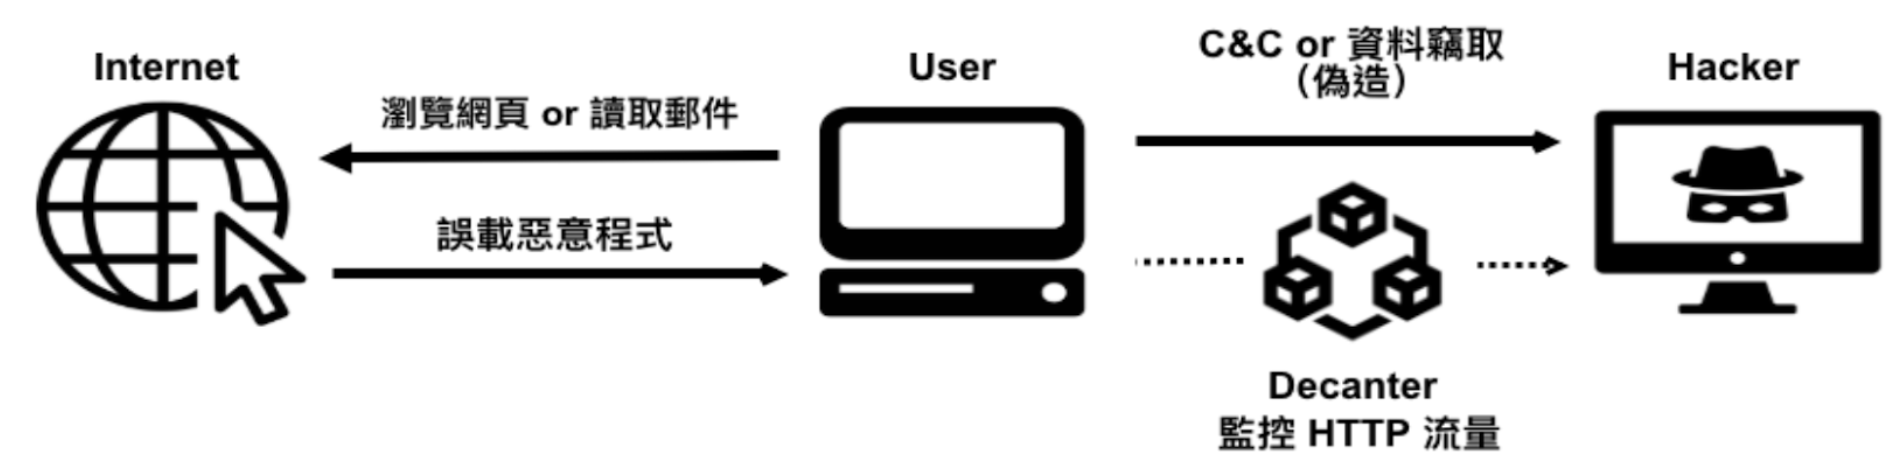
\includegraphics[width=250pt]{image/attack.png}
\caption{A process of attacking scenario}
\label{fig:attack}
\end{figure}


\begin{figure}[!tbp]
  \centering
  \subfloat[Normal Referrer Correlation Graph]{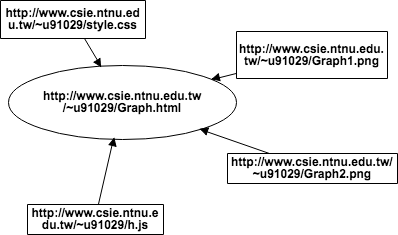
\includegraphics[width=0.25\textwidth]{image/normal.png}\label{fig:normal}}
  \hfill
  \subfloat[Malicious Referrer Correlation Graph]{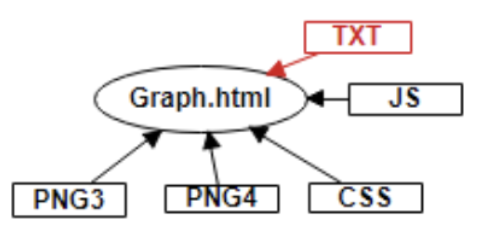
\includegraphics[width=0.25\textwidth]{image/malware.png}\label{fig:malware}}
  \caption{Difference between normal and malicious referrer correlation graph.}
\label{fig:length_count}
\end{figure}

Contributions of this work are briefly summarized as followings.

\begin{itemize}

\item {\bf Contribution 1}

Description here...

\item {\bf Contribution 2}

Description here...

\item {\bf Contribution 3}

Description here...

\end{itemize}